% Options for packages loaded elsewhere
\PassOptionsToPackage{unicode}{hyperref}
\PassOptionsToPackage{hyphens}{url}
%
\documentclass[
]{article}
\usepackage{amsmath,amssymb}
\usepackage{lmodern}
\usepackage{ifxetex,ifluatex}
\ifnum 0\ifxetex 1\fi\ifluatex 1\fi=0 % if pdftex
  \usepackage[T1]{fontenc}
  \usepackage[utf8]{inputenc}
  \usepackage{textcomp} % provide euro and other symbols
\else % if luatex or xetex
  \usepackage{unicode-math}
  \defaultfontfeatures{Scale=MatchLowercase}
  \defaultfontfeatures[\rmfamily]{Ligatures=TeX,Scale=1}
\fi
% Use upquote if available, for straight quotes in verbatim environments
\IfFileExists{upquote.sty}{\usepackage{upquote}}{}
\IfFileExists{microtype.sty}{% use microtype if available
  \usepackage[]{microtype}
  \UseMicrotypeSet[protrusion]{basicmath} % disable protrusion for tt fonts
}{}
\makeatletter
\@ifundefined{KOMAClassName}{% if non-KOMA class
  \IfFileExists{parskip.sty}{%
    \usepackage{parskip}
  }{% else
    \setlength{\parindent}{0pt}
    \setlength{\parskip}{6pt plus 2pt minus 1pt}}
}{% if KOMA class
  \KOMAoptions{parskip=half}}
\makeatother
\usepackage{xcolor}
\IfFileExists{xurl.sty}{\usepackage{xurl}}{} % add URL line breaks if available
\IfFileExists{bookmark.sty}{\usepackage{bookmark}}{\usepackage{hyperref}}
\hypersetup{
  pdftitle={A Bayesian Hidden Markov Model Approach to Resampled Frontiers},
  hidelinks,
  pdfcreator={LaTeX via pandoc}}
\urlstyle{same} % disable monospaced font for URLs
\usepackage[margin=1in]{geometry}
\usepackage{color}
\usepackage{fancyvrb}
\newcommand{\VerbBar}{|}
\newcommand{\VERB}{\Verb[commandchars=\\\{\}]}
\DefineVerbatimEnvironment{Highlighting}{Verbatim}{commandchars=\\\{\}}
% Add ',fontsize=\small' for more characters per line
\usepackage{framed}
\definecolor{shadecolor}{RGB}{248,248,248}
\newenvironment{Shaded}{\begin{snugshade}}{\end{snugshade}}
\newcommand{\AlertTok}[1]{\textcolor[rgb]{0.94,0.16,0.16}{#1}}
\newcommand{\AnnotationTok}[1]{\textcolor[rgb]{0.56,0.35,0.01}{\textbf{\textit{#1}}}}
\newcommand{\AttributeTok}[1]{\textcolor[rgb]{0.77,0.63,0.00}{#1}}
\newcommand{\BaseNTok}[1]{\textcolor[rgb]{0.00,0.00,0.81}{#1}}
\newcommand{\BuiltInTok}[1]{#1}
\newcommand{\CharTok}[1]{\textcolor[rgb]{0.31,0.60,0.02}{#1}}
\newcommand{\CommentTok}[1]{\textcolor[rgb]{0.56,0.35,0.01}{\textit{#1}}}
\newcommand{\CommentVarTok}[1]{\textcolor[rgb]{0.56,0.35,0.01}{\textbf{\textit{#1}}}}
\newcommand{\ConstantTok}[1]{\textcolor[rgb]{0.00,0.00,0.00}{#1}}
\newcommand{\ControlFlowTok}[1]{\textcolor[rgb]{0.13,0.29,0.53}{\textbf{#1}}}
\newcommand{\DataTypeTok}[1]{\textcolor[rgb]{0.13,0.29,0.53}{#1}}
\newcommand{\DecValTok}[1]{\textcolor[rgb]{0.00,0.00,0.81}{#1}}
\newcommand{\DocumentationTok}[1]{\textcolor[rgb]{0.56,0.35,0.01}{\textbf{\textit{#1}}}}
\newcommand{\ErrorTok}[1]{\textcolor[rgb]{0.64,0.00,0.00}{\textbf{#1}}}
\newcommand{\ExtensionTok}[1]{#1}
\newcommand{\FloatTok}[1]{\textcolor[rgb]{0.00,0.00,0.81}{#1}}
\newcommand{\FunctionTok}[1]{\textcolor[rgb]{0.00,0.00,0.00}{#1}}
\newcommand{\ImportTok}[1]{#1}
\newcommand{\InformationTok}[1]{\textcolor[rgb]{0.56,0.35,0.01}{\textbf{\textit{#1}}}}
\newcommand{\KeywordTok}[1]{\textcolor[rgb]{0.13,0.29,0.53}{\textbf{#1}}}
\newcommand{\NormalTok}[1]{#1}
\newcommand{\OperatorTok}[1]{\textcolor[rgb]{0.81,0.36,0.00}{\textbf{#1}}}
\newcommand{\OtherTok}[1]{\textcolor[rgb]{0.56,0.35,0.01}{#1}}
\newcommand{\PreprocessorTok}[1]{\textcolor[rgb]{0.56,0.35,0.01}{\textit{#1}}}
\newcommand{\RegionMarkerTok}[1]{#1}
\newcommand{\SpecialCharTok}[1]{\textcolor[rgb]{0.00,0.00,0.00}{#1}}
\newcommand{\SpecialStringTok}[1]{\textcolor[rgb]{0.31,0.60,0.02}{#1}}
\newcommand{\StringTok}[1]{\textcolor[rgb]{0.31,0.60,0.02}{#1}}
\newcommand{\VariableTok}[1]{\textcolor[rgb]{0.00,0.00,0.00}{#1}}
\newcommand{\VerbatimStringTok}[1]{\textcolor[rgb]{0.31,0.60,0.02}{#1}}
\newcommand{\WarningTok}[1]{\textcolor[rgb]{0.56,0.35,0.01}{\textbf{\textit{#1}}}}
\usepackage{graphicx}
\makeatletter
\def\maxwidth{\ifdim\Gin@nat@width>\linewidth\linewidth\else\Gin@nat@width\fi}
\def\maxheight{\ifdim\Gin@nat@height>\textheight\textheight\else\Gin@nat@height\fi}
\makeatother
% Scale images if necessary, so that they will not overflow the page
% margins by default, and it is still possible to overwrite the defaults
% using explicit options in \includegraphics[width, height, ...]{}
\setkeys{Gin}{width=\maxwidth,height=\maxheight,keepaspectratio}
% Set default figure placement to htbp
\makeatletter
\def\fps@figure{htbp}
\makeatother
\setlength{\emergencystretch}{3em} % prevent overfull lines
\providecommand{\tightlist}{%
  \setlength{\itemsep}{0pt}\setlength{\parskip}{0pt}}
\setcounter{secnumdepth}{-\maxdimen} % remove section numbering
\ifluatex
  \usepackage{selnolig}  % disable illegal ligatures
\fi

\title{A Bayesian Hidden Markov Model Approach to Resampled Frontiers}
\author{}
\date{\vspace{-2.5em}}

\begin{document}
\maketitle

\hypertarget{download-data}{%
\subsection{Download Data}\label{download-data}}

In this brief case study, I apply my Bayesian Hidden Markov Model (HMM)
implementation to an all-ETF portfolio allocation problem by proposing a
novel resampled efficient frontier idea based upon the posterior
predictive distribution of asset weights, arrived at through
mean-variance optimization. The Bayesian HMM resampled frontier
framework provides a coherent paradigm for incorporating both parameter
estimation uncertainty and market regime uncertainty into the
mean-variance optimization process. This is in contrast with the
certainty equivalence principal of standard mean-variance optimization,
whereby ``plug-in'' parameter estimates are used in the optimization
routine which can lead to badly-leveraged portfolio weights due the
inherent unaccounted uncertainties involved in the estimation process
{[}2{]}.

To start, I'll download weekly return data for a basket of five ETFs: 1.
S\&P 500 2. EFA -- a non-US equities fund 3. IJS -- a small-cap value
fund 4. EEM -- an emerging-markets fund 5. AGG -- a fixed income bond
fund.

\begin{Shaded}
\begin{Highlighting}[]
\NormalTok{symbols }\OtherTok{\textless{}{-}} \FunctionTok{c}\NormalTok{(}\StringTok{"SPY"}\NormalTok{,}\StringTok{"EFA"}\NormalTok{, }\StringTok{"IJS"}\NormalTok{, }\StringTok{"EEM"}\NormalTok{,}\StringTok{"AGG"}\NormalTok{)}

\NormalTok{prices }\OtherTok{\textless{}{-}} \FunctionTok{getSymbols}\NormalTok{(symbols, }\AttributeTok{src =} \StringTok{\textquotesingle{}yahoo\textquotesingle{}}\NormalTok{, }\AttributeTok{from =} \StringTok{"2005{-}01{-}01"}\NormalTok{,}
             \AttributeTok{auto.assign =} \ConstantTok{TRUE}\NormalTok{, }\AttributeTok{warnings =} \ConstantTok{FALSE}\NormalTok{) }\SpecialCharTok{\%\textgreater{}\%}
  \FunctionTok{map}\NormalTok{(}\SpecialCharTok{\textasciitilde{}}\FunctionTok{Ad}\NormalTok{(}\FunctionTok{get}\NormalTok{(.))) }\SpecialCharTok{\%\textgreater{}\%}
  \FunctionTok{reduce}\NormalTok{(merge) }\SpecialCharTok{\%\textgreater{}\%}
  \StringTok{\textasciigrave{}}\AttributeTok{colnames\textless{}{-}}\StringTok{\textasciigrave{}}\NormalTok{(symbols)}
\end{Highlighting}
\end{Shaded}

\begin{verbatim}
## 'getSymbols' currently uses auto.assign=TRUE by default, but will
## use auto.assign=FALSE in 0.5-0. You will still be able to use
## 'loadSymbols' to automatically load data. getOption("getSymbols.env")
## and getOption("getSymbols.auto.assign") will still be checked for
## alternate defaults.
## 
## This message is shown once per session and may be disabled by setting 
## options("getSymbols.warning4.0"=FALSE). See ?getSymbols for details.
\end{verbatim}

\begin{Shaded}
\begin{Highlighting}[]
\NormalTok{prices\_monthly }\OtherTok{\textless{}{-}} \FunctionTok{to.weekly}\NormalTok{(prices, }\AttributeTok{indexAt =} \StringTok{"last"}\NormalTok{, }\AttributeTok{OHLC =} \ConstantTok{FALSE}\NormalTok{)}
\NormalTok{asset\_returns\_xts }\OtherTok{\textless{}{-}} \FunctionTok{na.omit}\NormalTok{(}\FunctionTok{Return.calculate}\NormalTok{(prices\_monthly, }\AttributeTok{method =} \StringTok{"log"}\NormalTok{))}
\end{Highlighting}
\end{Shaded}

I'll visualize the collection of log-returns over time as follows

\begin{Shaded}
\begin{Highlighting}[]
\FunctionTok{matplot}\NormalTok{(asset\_returns\_xts[,], }\AttributeTok{type=}\StringTok{"l"}\NormalTok{, }\AttributeTok{ylab=}\StringTok{"log{-}return"}\NormalTok{, }\AttributeTok{xlab=}\StringTok{"Week"}\NormalTok{)}
\FunctionTok{legend}\NormalTok{(}\DecValTok{300}\NormalTok{,.}\DecValTok{2}\NormalTok{,}\AttributeTok{legend =}\NormalTok{ symbols[],}\AttributeTok{fill =} \DecValTok{1}\SpecialCharTok{:}\FunctionTok{length}\NormalTok{(symbols[]),}\AttributeTok{title =} \StringTok{"ETFs"}\NormalTok{, }\AttributeTok{cex=}\NormalTok{.}\DecValTok{7}\NormalTok{, }\AttributeTok{horiz =}\NormalTok{ T)}
\end{Highlighting}
\end{Shaded}

\begin{center}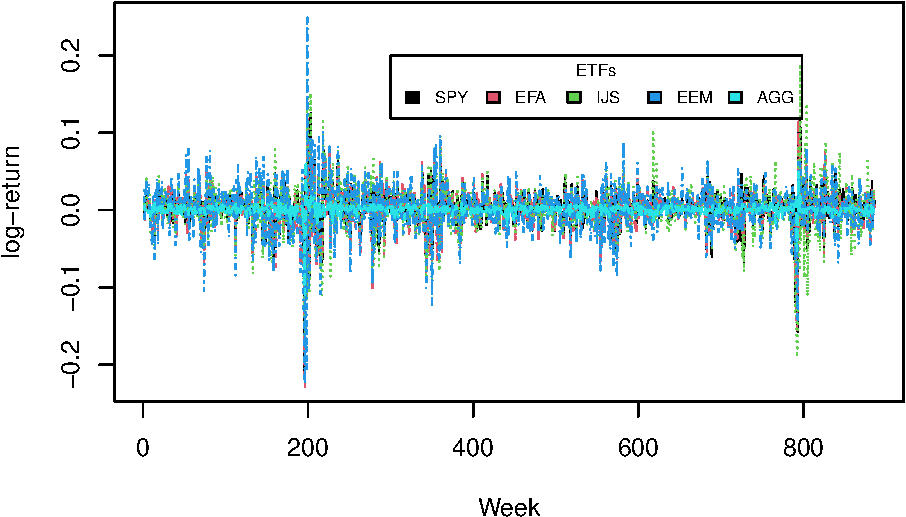
\includegraphics{portfolio_allocation_files/figure-latex/visual-1} \end{center}

To reframe the problem formally, I seek to solve the optimization
problem \[
\begin{equation}
  \begin{align}
  \min_{\omega} & & \omega^\top\Sigma_{T+\tau}\omega \\
  \text{subject to} &  &\omega^\top\mu_{T+\tau}\geq\mu^{\star}\\
  \text{and} & & \omega^\top1  = 1,
  \end{align}
\end{equation}
\] which implies minimizing portfolio variance while ensuring returns of
some level \(\mu^\star\). I'll employ the posterior predictive
distribution of the fitted HMM to obtain a probability distribution of
estimates for plausible portfolio weights \(\omega\) for the yet
unrealized time period \(T+\tau\), conditional only upon the return
series up to time \(T\). Sampling from the posterior predictive
distribution is algorithmicly straightforward through Monte Carlo
sampling as follows:

\begin{enumerate}
\def\labelenumi{\arabic{enumi}.}
\tightlist
\item
  Draw \(\Theta^{(s)}, S_{1:T}^{(s)}\sim p(\Theta, S_{1:T}|r_{1:T})\)
\item
  Draw \(S_{T+\tau}^{(s)}\sim p(S_{T+\tau}|S_T^{(s)}, \Theta^{(s)})\)
\item
  Solve (1) to draw from
  \(\omega^{(s)}_{T+\tau}\sim p(\omega_{T+\tau}|r_{1:T},\Theta^{(s)}, S_{T+\tau}^{(s)})\)
  for a given \(\mu^\star\)
\item
  Repeat 1-3 to form a collection of iid random draws from predictive
  density \(p(\omega_{T+\tau}|r_{1:T})\)
\end{enumerate}

Additionally, through this predictive density on
\(p(\omega_{T+\tau}|r_{1:T})\), I can obtain distributions for perfance
metrics such as, e.g., the Sharpe Ratio. Fraws from this distribution
\(p(SR^{(s)}|r_{1:T})\) can be computed through \[
SR^{(s)}:=\frac{\omega_{T+\tau}^{(s)\top}\mu_{T+\tau}}{\sqrt{\omega_{T+\tau}^{(s)\top}\Sigma_{T+\tau}\omega_{T+\tau}^{(s)}}}.
\]

Finally, the efficient frontier distribution can now be traced out for
given values of \(\mu^\star\) by then computing the portfolio risk
\(\sqrt{\omega_{T+\tau}^{(s)\top}\Sigma_{T+\tau}\omega_{T+\tau}^{(s)}}\)
for a given sample \(\omega_{T+\tau}^{(s)}\) from
\(p(\omega_{T+\tau}|r_{1:T})\).

\begin{Shaded}
\begin{Highlighting}[]
\NormalTok{sampler }\OtherTok{=} \ControlFlowTok{function}\NormalTok{(y, niter, burnin, mu0, Sigma0, v0, S0, m, nugget)\{}
\NormalTok{  r }\OtherTok{\textless{}{-}} \ConstantTok{NULL}
\NormalTok{  attempt }\OtherTok{\textless{}{-}} \DecValTok{1}
  \ControlFlowTok{while}\NormalTok{( }\FunctionTok{is.null}\NormalTok{(r) }\SpecialCharTok{\&\&}\NormalTok{ attempt }\SpecialCharTok{\textless{}=} \DecValTok{3}\NormalTok{ ) \{}
\NormalTok{    attempt }\OtherTok{\textless{}{-}}\NormalTok{ attempt }\SpecialCharTok{+} \DecValTok{1}
    \FunctionTok{try}\NormalTok{(}
\NormalTok{       r }\OtherTok{\textless{}{-}} \FunctionTok{gibbs}\NormalTok{(}\AttributeTok{niter =}\NormalTok{ niter, }\AttributeTok{burnin =}\NormalTok{ burnin,}
                      \AttributeTok{y =}\NormalTok{ y, }\AttributeTok{Sigma0 =}\NormalTok{ Sigma00, }\AttributeTok{v0 =}\NormalTok{ v0, }\AttributeTok{mu0 =}\NormalTok{ mu0, }\AttributeTok{S0 =}\NormalTok{ S0, }\AttributeTok{h=}\DecValTok{1}\NormalTok{, nugget, m)}
\NormalTok{    )}
\NormalTok{  \}}
  \FunctionTok{return}\NormalTok{(r)}
\NormalTok{\}}
\end{Highlighting}
\end{Shaded}

\begin{center}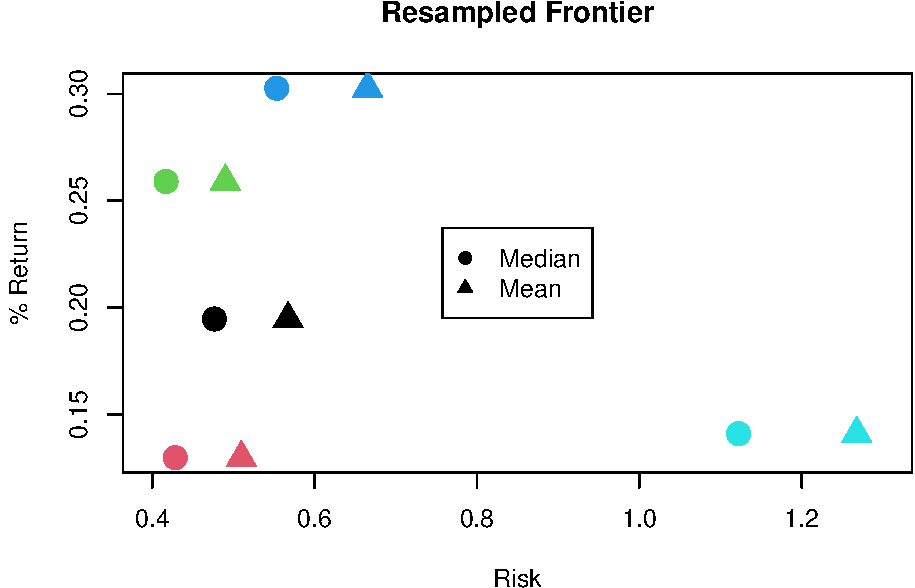
\includegraphics[width=8.5in]{portfolio_allocation_files/figure-latex/unnamed-chunk-3-1} \end{center}

\hypertarget{references}{%
\section{References}\label{references}}

\begin{itemize}
\tightlist
\item
  \href{https://faculty.fuqua.duke.edu/~charvey/Research/Published_Papers/P95_Bayes_vs_Markowitz.pdf}{\emph{Bayes
  vs.~Resampling: A Rematch}} - Harvey, Liechtyb and Liechtyc
\item
  \href{https://www.wiley.com/en-us/Bayesian+Methods+in+Finance-p-9780470249246}{\emph{Bayesian
  Methods in Finance}} - Rachev, Hsu, Bagasheva, and Fabozzi.
\item
  \href{https://link.springer.com/content/pdf/10.1007\%2F978-0-387-35768-3.pdf}{\emph{Finite
  Mixture and Markov Switching Models}} - Sylvia Fruhwirth-Schnatter.
\end{itemize}

\end{document}
